\section{Das McCulloch-Pitts-Neuron}\label{sec:mcpneuron}

Im Jahr 1943 veröffentlichen \textit{Warren McCulloch} und \textit{Walter Pitts} ihre Arbeit~\cite{MP43}.
Sie stellen darin ein auf \textbf{Aussagenlogik} basierendes mathematisches Modell zur Erklärung von Signalverarbeitung und  -weiterleitung im Nervensystem vor, und liefern damit grundlegende Ideen für die Kybernetik und die Von-Neumann-Rechnerarchitektur.
Ihre Arbeit leistet insgesamt einen wichtigen Beitrag für die Entwicklung \textit{Künstlicher Intelligenz}(vgl.~\cite[1]{Arb19}).


\subsection{Der Kalkül}\label{sec:mcpkalkül}

In der \textbf{Principia Mathematica} stellen \textit{Russel} und \textit{Bertrand} die Mathematik auf ein Gerüst logischer Grundprinzipien (vgl.~\cite[225]{She26}). Inspiriert dadurch beschäftigt sich McCulloch mit der Frage, ob es nicht auch möglich sei, die Vorgänge im Gehirn durch Anwendung logischer Prinzipien erklärbar zu machen (vgl.~\cite[4]{Arb19}). Die Zweiwertigkeit des Alles-oder-Nichts-Prinzips (siehe Abschnitt~\ref{sec:aktionspotenzial}) führt zu dem Kalkül:

\blockquote[{\cite[100]{MP43}}]{
    The `all-or-none law` of nervous activity is sufficient to insure that the activity of any neuron may be represented as a proposition.
}\\

McCulloch und Pitts gehen für ihren Kalkül von folgenden physischen Eigenschaften einer Nervenzelle aus (vgl.~\cite[101]{MP43}):


\begin{enumerate}
    \item Ein Neuron arbeitet auf Basis des Alles-oder-Nichts-Prinzip.
    \item Eine gewisse Anzahl von Synapsen muss innerhalb einer bestimmten Zeit angeregt werden, um ein Neuron zu erregen.
    \item Die einzige signifikante Verzögerung bei der Signalübertragung innerhalb des Nervensystems ist bedingt durch synaptische Verzögerungen.
    \item Eine einzige hemmende Synapse verhindert die Erregung des betreffenden Neurons.
    \item Die Struktur des neuronalen Netzes ändert sich nicht.
\end{enumerate}


\subsection{Anwendung des Modells}
Das in diesem Abschnitt vorgestellte Modell soll - in Anlehnung an die Arbeit von McCulloch \& Pitts - folgende Anforderungen erfüllen\footnote{
    vgl.~\cite[26 f.]{Fau94}. Für unsere einführende Betrachtung folgen wir~\cite[33 f.]{Roj93} und ignorieren zunächst die Zeitwerte aus der Original-Arbeit: Dort wird für die Signalübertragung ein diskreter Zeitwert $t \in \mathbb{Z}$ vereinbart: Die Übertragung eines Signals dauert eine Zeiteinheit, also $t + 1$. Vgl. hierzu Abbildung~\ref{fig:mcpcell}.
}
\begin{enumerate}
    \item Das Verhalten des künstlichen Neurons ist zweiwertig, also \textit{binär}. Das Neuron feuert, oder es feuert nicht. Im Sinne der Beziehung zwischen Eingabe und Ausgabe verstehen wir unter ``feuern`` den Wert $1$. Wenn ein Neuron nicht feuert, wird dies durch den Wert $0$ repräsentiert, der ebenfalls als Ausgabe vorliegt. In diesem Sinne produziert unser Modell also immer ein ``Signal``.
    \item An einem Neuron liegen (beliebig viele) Eingaben an.
    \item {
        Jedes Neuron hat einen individuellen Schwellenwert.
        Der Schwellenwert muss getroffen oder übertroffen werden, damit ein Neuron eine ``1`` feuert.
    }
    \item Hemmung ist ``absolut``: Liegt ein hemmendes Signal zusammen mit nicht-hemmenden Signalen an, feuert das Neuron nicht.
\end{enumerate}


\begin{figure}[h]
    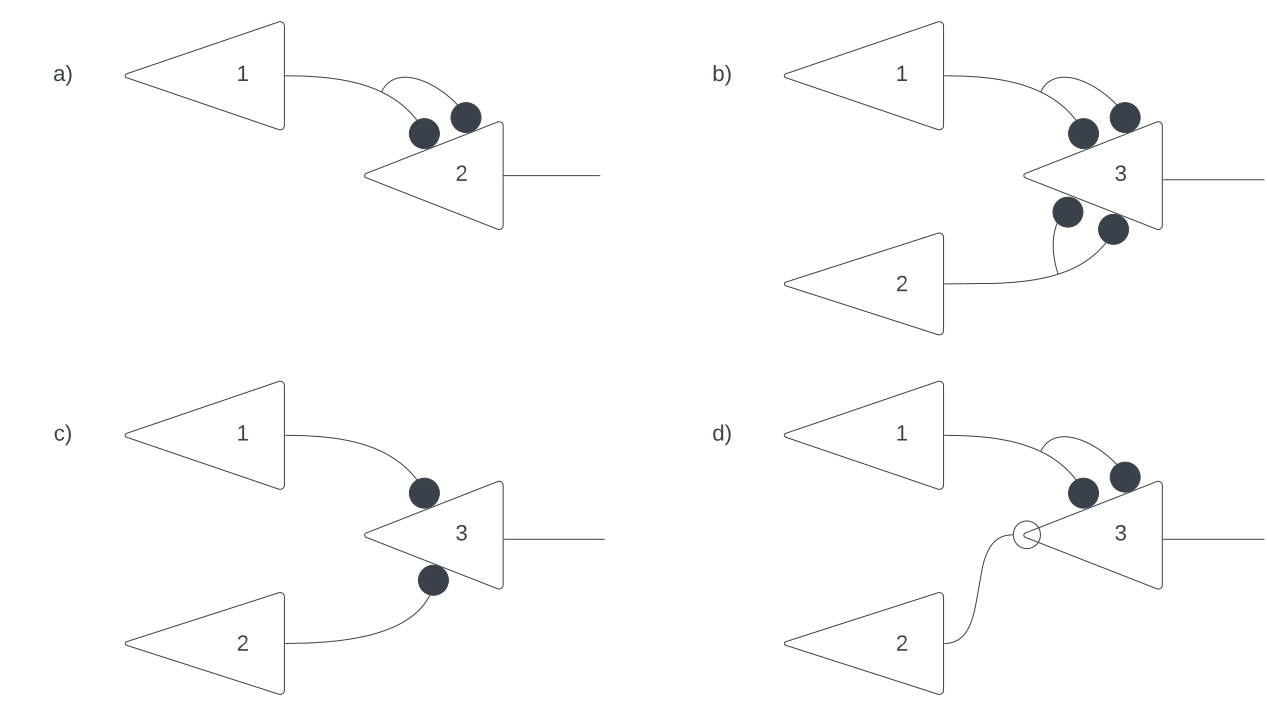
\includegraphics[
        width=16cm,
        keepaspectratio,
    ]{chapters/3. Kuenstliche Neuronen/images/mcpneuron}
    \caption{Schematische Darstellung von MCP-Zellen (Quelle: in Anlehnung an~\cite[105, Figure 1]{MP43})}
    \label{fig:mcpcell}
    \small{
     Schwarze Kreise sind erregende Verbindungen, offene Kreise hemmende. Im ursprünglichen Modell benötigt ein Neuron zwei erregende Eingaben, um aktiviert zu werden.\\
    In a) ist damit ein Netz dargestellt von zwei Neuronen, bei denen $N_2$ feuert, wenn $N_1$ feuert. Unter Berücksichtigung der Zeiteinheit folgt die formale Darstellung $N_2(t) \equiv N_1(t - 1)$.\\
    Gleicherweise ergibt sich für b), das $N_3$ nur feuert, wenn $N_1$ \textbf{oder} $N_2$ feuern: $N_3(t) \equiv N_1(t - 1) \lor N_2(t - 1)$.\\
    Analog folgt für c) $N_3(t) \equiv N_1(t - 1) \land N_2(t - 2)$.\\
    Für d) ergibt sich somit $N_3(t) \equiv N_1(t - 1 ) \land \neg N_2(t - 1)$
    }
\end{figure}


\subsection{Aktivierungs- und Eingabefunktion}\label{mcp-inputactivfunc}

Mit $n \in  \mathbb{N}_0$ und $m \in  \mathbb{N}_0$ wird festgelegt, dass ein Neuron $n + m$ Eingaben haben soll, mit $n \geq 1 \lor m \geq 1$, wobei $n$ die Anzahl der erregenden und $m$ die der hemmenden Eingaben ist.

Für die Schwellenwertfunktionen eines Neurons $N$ ergeben sich folgende Anforderungen: Die Summe der erregenden Eingabesignale $x_1, x_2, ..., x_n$ und der hemmenden Eingabesignale $y_1, y_2, ..., y_m$  muss den für das Neuron festgelegten Schwellenwert $\Theta \in  \mathbb{N}_0$ treffen oder überschreiten, damit als Ausgabe eine $1$ erzeugt wird, ansonsten liefert die Funktion eine $0$ zurück.

\subsection*{Eingabefunktion}
Zur Integration der eingehenden Signale wird eine \textbf{Eingabefunktion} benötigt.
Der Wert dieser Eingabefunktion wird dann auf eine Funktion angewendet, die entscheidet, ob das Neuron feuert oder nicht - also eine $1$ oder $0$ ausgibt.\\

\noindent
Für die Eingabesignale $X$

\begin{equation}
X \in \{1, 0\}^{n+m} \coloneqq (x_1, x_2 ..., x_n, y_1, y_2, ... y_m)
\end{equation}\linebreak[2]

\noindent
definieren wir die \textit{Gewichte} $w_+ \in \{2, 1\}$ mit $w^1_+ \coloneqq1, w^2_+ \coloneqq 2$ für erregende Signale, $w_- \coloneqq -1$ für hemmende Signale (vgl.~\cite[27-28]{Fau94}).\\


\noindent
Die \textbf{Eingabefunktion} $g$

\begin{equation}
g: \{1, 0\}^{n+m} \to  \mathbb{Z}, X \mapsto \sum^n_{j=1} x_jw_+ + \sum^m_{k=1} y_kw_-
\label{eq:gl-mcpinpfunc}
\end{equation}\linebreak[2]

\noindent
liefert die Summe der hemmenden und erregenden Eingabesignale zurück.


\subsection*{Aktivierungsfunktion}
Die Schwellenwertfunktion wird im Kontext von künstlichen neuronalen Netzen auch \textbf{Aktivierungsfunktion} genannt (vgl. ~\cite[847]{RN09}), da sie entscheidet, ob einzelne Neuronen aktiviert werden oder nicht.
In diesem Fall wird sie als \textbf{Treppenfunktion} realisiert, die $1$ zurückliefert, falls $g(X) >= \Theta$, und $0$ sonst :

\begin{equation}
f:  \mathbb{Z} \to \{0, 1\}, f(g(X)) = f(u) = \begin{cases}
                                          1  &\text{falls } u >= \Theta \\
                                          0 &\text{falls } u < \Theta
\end{cases}
\label{eq:gl-activation}
\end{equation}\linebreak[2]

\begin{figure}[h]
    \centering
    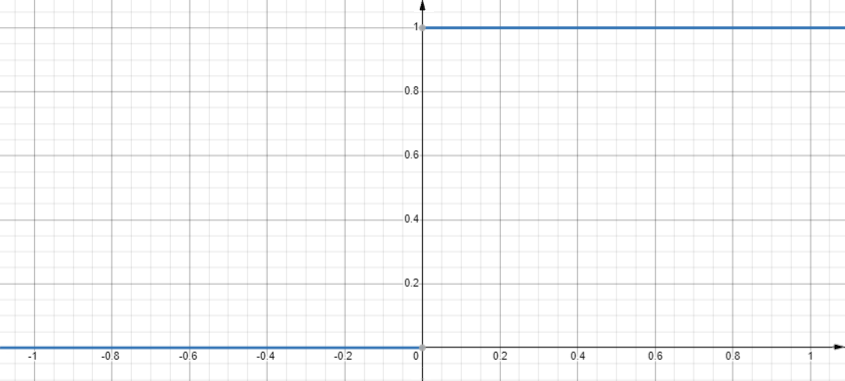
\includegraphics[
        width=12cm,
        keepaspectratio,
    ]{chapters/3. Kuenstliche Neuronen/images/heaviside}
    \caption{Plot einer Treppenfunktion, hier als Heaviside-Funktion mit $H\left(x\right)=\left\{x<0\ :\ 0,\ x\ge0\ :\ 1\right\}$. (Quelle: Eigene Darstellung)}
    \label{fig:heaviside}
\end{figure}


\noindent
Da die Erregung absolut ist, muss $\Theta$ die Ungleichung

\begin{equation}
\Theta > (\sum^{k^{w_+^2}}_{j=1} 2) + (\sum^{k^{w_+^1}}_{j=1} 1) + w_-
\end{equation}\linebreak[2]



\noindent
erfüllen, was abgekürzt werden kann zu

\begin{equation}
\Theta > 2k^{w_+^2} + k^{w_+^1} - 1
\end{equation}





\subsection{Modellierung der booleschen XOR-Funktion}\label{seq-mcpbool}

\setlength{\tabcolsep}{1.5em}
{\renewcommand{\arraystretch}{1.5}%
\begin{table} %[hbtp]
    \centering
    \begin{tabular}{c | c | c}
        $A$ & $B$ & $A \oplus B$ \\
        \hline
        1   & 1   & 0           \\
        1   & 0   & 1           \\
        0   & 1   & 1           \\
        0   & 0   & 0           \\
    \end{tabular}
    \caption{Die Wahrheitstabelle für \textbf{XOR}}
    \label{tab:xor}
\end{table}

\begin{figure}[h]
    \centering
    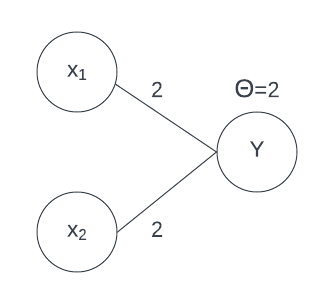
\includegraphics{chapters/3. Kuenstliche Neuronen/images/mcpor}
    \caption{Ein MCP-Neuron zur Modellierung von \textbf{OR} (Quelle: Eigene Darstellung)}
    \label{fig:mcpor}
\end{figure}

Für die Konstruktion eines Netzes zur Modellierung von \textbf{XOR} hilft zunächst das in Abbildung~\ref{fig:mcpor} dargestellte Modell der \textbf{OR}-Funktion. Der Schwellenwert ($\Theta = 2$) wird erreicht, wenn entweder $x_1$ oder $x_2$ ein erregendes Signal weiterleitet.
Allerdings wird der Schwellenwert auch erreicht, wenn jeweils $x_1$ \textit{und} $x_2$ gleichzeitig aktiv sind, denn dann ist $f_{xor}(g(X)) = 4$.
Also muss eine Hemmung zwischengeschaltet werden (s. Abbildung~\ref{fig:mcpxorf}): Ein aktives $x_1$ hemmt $N_2$. $N_2$ leitet in dem Fall $0$ an $Y$ weiter.
Die Zellen $x_2$ und $N_1$ werden analog verbunden.

Die \textbf{disjunktive Normalform} (Gleichung~\ref{eq:gl-xordis}) und die \textbf{konjunktive Normalform} (Gleichung~\ref{eq:gl-xorcon}) von \textbf{XOR} liefern die Formel für das Netz.
Insbesondere die disjunktive Normalform ist in Abbildung~\ref{fig:mcpxorf} erkennbar.\\

\begin{equation}
A \oplus B \equiv (\neg A \land B) \lor (A \land \neg B)
\label{eq:gl-xordis}
\end{equation}

\begin{equation}
A \oplus B \equiv (A \lor B) \land (\neg A \lor \neg B)
\label{eq:gl-xorcon}
\end{equation}


\begin{figure}[h]
    \centering
    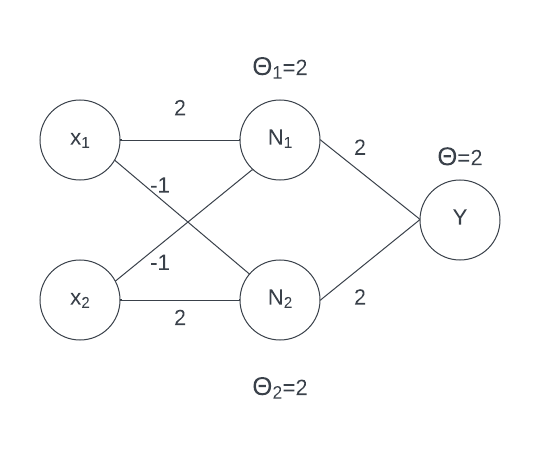
\includegraphics{chapters/3. Kuenstliche Neuronen/images/mcpxor}
    \caption{Entwurf für ein MCP-Netz zur Modellierung von \textbf{XOR}}
    \label{fig:mcpxorf}
\end{figure}









